%==========================================================================================================================================================================================

\section{Propuesta original}
    % [Describir la propuesta original hecha a la cátedra en esta sección, sobre todo desde el punto de vista funcional y agregar la propuesta original completa como Apéndice A de este informe]
    
    La propuesta original de este proyecto, se basa en el desarrollo de un programa para el microcontrolador Wemos D1 que le permita controlar una matriz de luces. La matriz está compuesta por módulos de 8x8 LEDs cada uno. Adicionalmente, el Wemos D1 debe ser capaz de hostear un servidor web, del cual extrae las peticiones HTTP que le realizan los clientes en relación al contenido que desean mostrar sobre la matriz.
    
    Respecto de las peticiones, éstas se clasifican en tres categorías: frases, mapeos led a led (explicitando cuáles de ellos deben estar encendidos y cuáles no), y por último la representación de sprites animados almacenados dentro de la memoria del microcontrolador.
    
    Como parte de la propuesta original es necesario, además, que el servidor previamente mencionado, corra sobre una red WiFi que el propio microcontrolador hostea y a la que se conectan los clientes. En otras palabras, el Wemos D1 debe actuar como access point. La tecnología implementada sobre el microcontrolador restringe una conexión máxima de cuatro clientes simultáneos.
    
    Para este proyecto se propusieron dos objetivos secundarios. En primer lugar una funcionalidad para que el dueño del sistema filtre las publicaciones que no desea mostrar en la matriz. El otro objetivo consiste en que el programa debe ser capaz de poder deslizar el contenido publicado en la matriz, al estilo marquesina, en caso de que el usuario así lo desease, por ejemplo si el mensaje fuese más largo que la cantidad de módulos de LEDs disponibles. En el apéndice \ref{Apendix:propuesta} se encuentra la propuesta aprobada por la cátedra.
    
    
    
%==========================================================================================================================================================================================
    
\section{Correcciones/cambios de la propuesta}


    \subsection{Indicadas por la Cátedra}
    % [Tal como las recibieron, en el caso de haber aclaraciones, compaginarlas]
    
    Las aclaraciones fueron, por un lado utilizar el Wemos D1 como Access Point y por otro, que la implementación del producto sobre la remera no era necesario; siendo prioritario el funcionamiento de la matriz de leds individualmente.
    
    
    \subsection{Definidas por el avance y disponibilidad}
    % [Enunciarlas y explicar las razones correspondientes]
    
    Para armar la matriz de LEDs se optó por utilizar dispositivos integrados shifters MAX7219 en vez de los 74HC595 ya que facilitan la multiplexación. Se compraron tres en total, los cuales tienen un costo de \$45 pesos cada uno. Por otro lado se optó por la utilización de LEDs individuales en sustitución de la tira de LEDs debido a la sugerencia de la cátedra respecto de construir un cartel aislado en vez de hacerlo sobre una remera.
    
    
    % [Tener en cuenta que de lo que describan en la sección anterior y en ambas subsecciones de esta sección debería quedar claro el proyecto entregado]
    
    Cabe destacar que los objetivos principales descriptos en la sección anterior se desarrollaron de manera completa y satisfactoriamente, en tiempo y forma.
    
    Respecto del objetivo secundario relacionado a la funcionalidad que permite administrar los posteos, se diseñó una interfaz para habilitar y deshabilitar las publicaciones que realicen los clientes. Adicionalmente, en la misma página, se agregaron interfaces gráficas para cambiar las intensidades de los LEDs y limpiar la pantalla, eliminado la última publicación. Estas herramientas se desarrollaron en tiempo y forma. El otro objetivo secundario que permite deslizar el contenido de la publicación a modo de marquesina se desarrolló completamente, en tiempo y forma. Adicionalmente se agregó un servidor DNS que corre sobre el microcontrolador a fin de mejorar la experiencia de usuario. Esta funcionalidad evita que el cliente deba recordar la dirección IP del servidor web hosteado por el Wemos D1.
    
    Por otra parte, respecto de la construcción de la matriz; se desarrolló un prototipo de dos módulos de 8x8 LEDs cada uno. La idea de crear más de un módulo tiene como objetivo hacer un especial énfasis respecto de la escalabilidad del proyecto, a fin de mostrar la facilidad, a nivel de software y hardware, para agregar más módulos de LEDs. El prototipo se construyó a modo de shield para que se integre pin a pin en el Wemos D1.
    
    
    
%==========================================================================================================================================================================================

\section{Descripción y documentación general}
    % [Diagrama esquemático de conexiones – cableado. Asociado a cada esquemático de conexiones agregar una foto del sistema real en la que se vean las conexiones del esquemático tal como las implementaron] [Debería mostrarse un esquemático general, describiendo todo el sistema, con su foto asociada, y un esquemático por cada subsistema, en particular el que involucre a la placa de desarrollo utilizada] [Opcionalmente, se puede agregar un video en el que se describa todo lo anterior. Este video opcional no reemplaza lo anterior sino que lo complementa.


    \subsection{Wemos D1} \label{sec:Wemosd1}
    El Wemos D1 está compuesto de un chip ESP8266 que posee conexión WiFi. El chip está montado sobre una placa Arduino compatible. En la figura \ref{fig:Wemos-plaqueta} se puede observar una imagen del microcontrolador provisto por la cátedra.
    
    \begin{figure}[ht!]
        \centering
        \begin{center}
            \includegraphics[width=0.9\textwidth]{FINAL/imagenes/wemos.jpg}
            \caption{Microcontrolador Wemos D1.}
            \label{fig:Wemos-plaqueta}
        \end{center}
    \end{figure}
    
    Las caracterísitcas principales de la placa se listan a continuación.
    \begin{itemize}
        \item Once entradas/salidas digitales.
        \item Una entrada analógica.
        \item Conector micro USB
        \item Distribución de pines tipo Arduino UNO.
        \item PWM en todos sus pines digitales.
        \item Voltaje de operación de 3.3 V
        \item Once pines digitales de entrada y salida.
        \item Frecuencia de clock de 80Mhz.
        \item Flash de 4MB.
        \item Dentro de la flash, 1MB reservado para el almacenamiento de archivos permanentes (SPIFFS).
    \end{itemize}
    
    En la tabla \ref{table:wemos-pin} se muestra la distribución de pines de la placa. Como se puede observar, soporta los protocolos de comunicación serie I2C y SPI, siendo este último, el utilizado en este proyecto para establecer la transmisión de mensajes entre el microcontrolador y los chips MAX7219 que manejan la matriz de LEDs.
    
    \begin{table}[ht]
        \centering
        \caption{Tabla pines Wemos D1.}
        \label{table:wemos-pin}
        \begin{tabular}{ccc}
        \hline
            Pin     & Función                   & ESP8266 pin \\ \hline
            D0      & RX                        & GPIO3       \\
            D1      & TX                        & GPIO1       \\
            D2      & IO                        & GPIO16      \\
            D3(D15) & IO, SCL                   & GPIO5       \\
            D4(D14) & IO, SDA                   & GPIO4       \\ 
            D5(D13) & IO, SCK                   & GPIO14      \\
            D6(D12) & IO, MISO                  & GPIO12      \\
            D7(D11) & IO, MOSI                  & GPIO13      \\
            D8      & IO, Pull up               & GPIO0       \\
            D9      & IO, Pull up, BUILDTIN LED & GPIO12      \\
            D10     & IO, Pull down, SS         & GPIO15      \\
            A0      & Entrada analógica         & A0          \\ \hline
        \end{tabular}
    \end{table}
    
    Tanto el convertidor analógico digital que posee la placa, como los pines de salida, tienen un valor lógico alto de 3.3 V. 
    
    Por otra parte, el microcontrolador es capaz de trabajar en tres modos de operación. Puede actuar como cliente WiFi, como access point o como ambas. Adicionalmente esta placa soporta la programación OTA (Over The Air).
    

    \subsection{MAX7219}

        \subsubsection{Descipción general}
        El MAX7219 es un controlador compacto, de entrada y salida en serie de cátodo común que conectan microprocesadores a LEDs numéricos de siete segmentos de hasta ocho dígitos, pantallas de gráfico de barras o 64 LED individuales. Se incluyen en el chip, un decodificador BCD, circuitos de multiplexación, controladores de segmentos y dígitos, y una RAM estática de 8x8 que almacena cada número. Solo se necesita una resistencia externa para configurar la corriente de segmento para todos los LEDs.
        
        El MAX7219 es compatible con los protocolos SPI, QSPI y Microwire, y tiene controladores de segmento de velocidad limitada para reducir el EMI.
        
        Los dígitos individuales se pueden actualizar sin reescribir toda la pantalla. El MAX7219 también permite al usuario seleccionar el código de decodificación o no decodificación para cada dígito.
        
        Su alimentación V\texttt{+} debe estar entre 4 y 5.5 Volts para su correcto funcionamiento. En cambio los voltaje de las entradas lógicas tienen una restricción de que un valor alto como mínimo debe ser 3.5V y un valor bajo como máximo 0.8V. Como la placa usada tiene valores digitales de 3.3V, se realizaron previamente las pruebas necesarias para llegar a la conclusión de que, mas allá de la restriccion del datasheet, la placa utilizada logra comunicarse con el MAX7219 de forma correcta en todos los casos. 
        
        Las características principales que posee el chip integrado se enumeran a continuación:
        \begin{itemize}
            \item Interfaz serie de 10 MHz.
            \item Control de segmento LED individual.
            \item Selección de dígitos Decode / No-Decode.
            \item Apagado de baja potencia de 150 microA (datos retenidos).
            \item Control de brillo digital y analógico.
            \item Pantalla borrada al encenderse.
            \item Unidad de visualización LED de cátodo común.
            \item SPI, QSPI, interfaz serie Microwire paquetes DIP y SO de 24 pines.
        \end{itemize}


        \subsubsection{Configuración de pines}
        La disposición de los pines del MAX7219 se puede observar en la figura \ref{fig:MAX-pines} y la descripción de cada uno en la tabla \ref{table:MAX-pines}.
        
        Es necesario prestar atención en el conexionado con respecto a los pines de tierra (GND) ya que ambos deben estar conectados para el driver pueda funcionar correctamente, ambas estan al lado izquierdo de la figura \ref{fig:MAX-pines} (Pin 4 y 9).
        
        Por otro lado, el MAX7219 tiene un pin denominado DOUT (pin 24) se utiliza para encadenar varios MAX7219 y de esta forma pasar la información al que esta directamente conectado, éste pin nunca tiene alta impedancia.\\
        
        \begin{figure}[ht!]
            \centering
            \begin{center}
            \includegraphics[scale=1.2]{imagenes/hw-conexiones/max.pdf}
             \caption{Configuración de pines del chip MAX7219.}
              \label{fig:MAX-pines}
            \end{center}
        \end{figure}
        
\begin{table}[ht]
\centering
\caption{Descripción de los pines del MAX7219}
\label{table:MAX-pines}
\begin{tabular}{C{10mm} C{14mm} L{108mm}}
\hline
Pin               & Nombre          & Función    \\ \hline
1                 & DIN             & Pin de datos seriales. Los datos son cargados en el registro de 16 bits en cada flanco ascendente del clock. \\
2, 3, 5–8, 10, 11 & DIG 0 - DIG 7    & Líneas de transmisión de ocho dígitos que absorben corriente del cátodo común de la pantalla. El MAX7219 deja en V+ cuando esta apagado. Los dígitos están en alta impedancia cunado se apaga.\\
4, 9              & GND             & Tierra.\\
12                & LOAD            & Pin de control. Los últimos 16 bits del Serial Data son cargados en el flanco ascendente. \\
13                & CLK             & Pin de clock serial. En cada flanco ascendente, los datos sin shifteados dentro de un registro interno. En cada flanco descendente los datos salen de DOUT. En el MAX7221, la entrada CLK está activa solo mientras LOAD está baja. \\
14–17, 20-23      & SEG A–SEG G, DP & Las unidades de siete segmentos y el punto decimal impulsan la fuente de corriente a la pantalla. Cuando un controlador de segmento está apagado, se conecta a GND.\\
18                & ISET            & Conectar a  $V_{DD}$ a través de una resistencia ($R_{SET}$) para configurar la corriente que pueda entregar a los dígitos y segmentos. \\
19                & V+              & Fuente positiva de corriente, conectar a 5 V. \\
24                & DOUT            & Salida de datos en serie. Los datos en DIN son válidos en DOUT 16.5 ciclos de reloj más tarde. \\ \hline
\end{tabular}
\end{table}

    \subsection{Alimentación}
    Para la alimentación del microcontrolador se utilizará un PowerBank conectado vía USB (5V) a la placa del Wemos D1. La batería mencionada será la única fuente de alimentación del sistema.
    
    La alimentación de 5V para los integrados MAX7219 se extraerá del Wemos D1, ya que posee pines para dicho propósito. Este integrado se conecta a 5V por el pin VCC (ver figura \ref{fig:Wemos-MAX}), y es recomendado incluir capacitores electrolíticos para ayudar a desacoplar la línea de alimentación y absorber los picos transitivos de energía necesarios para encender y apagar los LEDs.
    

    \subsection{Conexión del Wemos D1 con el MAX7219}
    El microcontrolador se conecta con un chip shifter MAX7219 de la forma en que se muestra en la figura \ref{fig:Wemos-MAX}.
    
    El microcontrolador Wemos D1 soporta el protocolo de comunicación serie SPI, como ya se describió en la sección \ref{sec:Wemosd1}. Para ello se utiliza los pines D13 (SCK), D11 (MOSI) y D10 (SS) para el clock, datos y load respectivamente que se conectan directamente a las entradas del shifter MAX7219 tal como se puede observar en la figura \ref{fig:Wemos-MAX}.

    Adicionalmente, en la figura \ref{fig:Wemos-MAX-real} se observa una foto del Wemos D1 y sus conexiones con el MAX7219. A fin de facilitar la comprensión del circuito, se utilizan cables de colores donde cada uno de ellos representa una funcionalidad. Se utiliza el verde para la conexión con Vcc y el rojo para ground. Mientras que para el clock, datos y load se utilizan los cables amarillo, gris y azul respectivamente.

    \begin{figure}[ht!]
        \centering
        \begin{center}
            \includegraphics[width=0.66\textwidth]{imagenes/hw-conexiones/conexion-Wemos-MAX.pdf}
            \caption{Conexión del microcontrolador Wemos D1 con MAX7219.}
            \label{fig:Wemos-MAX}
        \end{center}
    \end{figure}
    
    \begin{figure}[ht!]
        \centering
        \begin{center}
            \includegraphics[width=0.6\textwidth]{imagenes/hw-conexiones/conexion-Wemos-MAX.JPG}
            \caption{Fotografía de interconexión del microcontrolador Wemos D1 con MAX7219.}
            \label{fig:Wemos-MAX-real}
        \end{center}
    \end{figure}


    \subsection{Conexión del MAX7219 con su módulo de 8x8 LEDs}
    Cada uno de los MAX7219 está conectado a un módulo de de 8x8 LEDs, sus conexiones se pueden observar en el diagrama \ref{fig:MAX-matriz}. Adicionalmente, en la figura \ref{fig:MAX-matriz-real} se observa el prototipo que complementa el esquema de conexión de la figura previamente mencionada. 
    
    A la hora de efectuar las conexiones, se debe prestar principal atención a la orientación de la matriz. En la figura \ref{fig:MAX-matriz-real} se indica claramente cuáles son las filas (y su orden) y cuáles son las columnas. Con dicha información el proceso de conexionado se simplifica.

    \begin{figure}[ht!]
        \centering
        \begin{center}
            \includegraphics[width=0.7\textwidth]{imagenes/hw-conexiones/conexion-MAX-matriz.pdf}
            \caption{Conexión entre MAX7219 y su módulo de LEDs.}
            \label{fig:MAX-matriz}
        \end{center}
    \end{figure}
    
    \begin{figure}[ht!]
        \centering
        \begin{center}
            \includegraphics[width=0.6\textwidth]{imagenes/hw-conexiones/conexion-MAX-matriz.JPG}
            \caption{Fotografía de conexión entre MAX7219 y su módulo de LEDs.}
            \label{fig:MAX-matriz-real}
        \end{center}
    \end{figure}


    \subsection{Concatenación de varios módulos de LEDs}
    Anteriormente se hizo referencia a la forma en que se conectan el Wemos D1 con un MAX7219 y a la manera en que éste lo hace con la matriz de LEDs. Sin embargo al inicio del informe se mencionó la posibilidad de interconectar más de un módulo de 8x8 LEDs. En particular, para este proyecto se conectan dos módulos, generando una matriz de 8 filas por 16 columnas, dando un total de 128 luces.

    Para realizar esta operación, es necesario que los MAX7219 se interconecten, uniendo el pin Data-Out del primero, hacia el pin Data-In del siguiente. Ésto permite que la información circule entre un shifter y el otro, de manera serial. Cabe mencionar que cada módulo funcional, está conectado al pin de clock y load del Wemos D1 para la transferencia de datos de forma serial.
    
    Es importante aclarar que la forma en la que se comunica un MAX7219 con el siguiente se detalla en la sección \ref{sec:comunicacion}. En esta parte solo se especifica el conexionado para que pueda establecerse el pasaje de los datos entre un chip y el siguiente.
    
    Por otra parte, a fin de conocer el consumo máximo de un chip shifter MAX7219 conectado con su respectivo módulo de 8x8 LEDs, se utilizaron las ecuaciones proporcionadas en el \href{https://datasheets.maximintegrated.com/en/ds/MAX7219-MAX7221.pdf}{link} del chip. Éstas fórmulas contemplan las variables donde puede llegar a producirse mayor incertidumbre. Se obtuvo un consumo de 8.5 mA por módulo.

    En la figura \ref{fig:MAX-MAX} se observa la forma en que se debe realizar la interconexión de los dispositivos integrados previamente mencionados mientras que la figura \ref{fig:MAX-MAX-real} complementa el esquemático mostrando una fotografía real del prototipo funcional.
    
    Para la fotografía, se quitaron determinados cables a fin de simplificar el esquema. Sólo se dejaron los necesarios para mostrar como se conectan dos MAX7219. Los colores se mantienen iguales respecto de la figura \ref{fig:Wemos-MAX-real}. Se puede observar que el cable blanco se conecta desde el pin DataOut del primer MAX7219 hacia el pin DataIn del segundo. Por otra parte el clock y load se comparten con el primer shifter cuyos colores son amarillo y azul respectivamente.

    \begin{figure}[ht!]
        \centering
        \begin{center}
            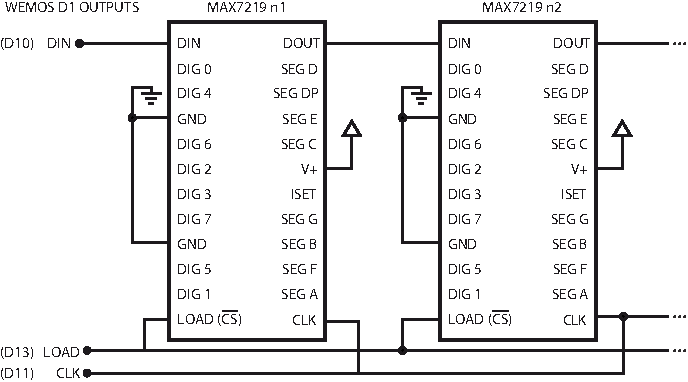
\includegraphics[width=\textwidth]{imagenes/hw-conexiones/MAX-daisychain.pdf}
            \caption{Conexión entre dos MAX7219.}
            \label{fig:MAX-MAX}
        \end{center}
    \end{figure}
    
    \begin{figure}[ht!]
        \centering
        \begin{center}
            \includegraphics[width=1\textwidth]{imagenes/hw-conexiones/conexion-MAX-MAX.JPG}
            \caption{Fotografía de conexión entre dos MAX7219.}
            \label{fig:MAX-MAX-real}
        \end{center}
    \end{figure}


    \subsection{Conexionado de LEDs y armado de la matriz}
    Los LEDs color blanco soportan entre 2.8V a 4.2V con una corriente de 20mA, por lo que se eligió un tensión promedio de 3V para alimentarlos. La hoja de datos del dispositivo integrado MAX7219 indica que es necesario colocar una resistencia $R_{SET}$ entre el pin $I_{SET}$ y la alimentación para controlar la tensión y la corriente entregada en sus pines de salida. A fin de obtener más claridad, respecto del nombre de los pines, se puede observar la figura \ref{table:MAX-pines} la configuración de los pines del shifter. La tabla \ref{table-RIsec} permite elegir $R_{SET}$ según las necesidades de cada aplicación o sistema; para este proyecto se eligió $R_{SET}$ con valor de 24.5KOhm aproximadamente debido a las características previamente enunciadas de los LEDs utilizados para cada módulo.\newline

    \begin{table}[ht]
        \centering
        \caption{Tabla extraída del \href{https://datasheets.maximintegrated.com/en/ds/MAX7219-MAX7221.pdf}{datasheet} del MAX7219, que relaciona la resistencia $R_{SET}$ con la salida de sus pines.}
        \vspace{2mm}
        \label{table-RIsec}
        \begin{tabular}{|c|ccccc|}\hline
        \multirow{2}{*}{$I_{SET}$(mA)} & \multicolumn{5}{c|}{$V_{LED}$(V)}   \\ \cline{2-6}
                    & 1.5  & 2.0  & 2.5  & 3.0  & 3.5  \\ \hline
        40          & 12.2 & 11.8 & 11.0 & 10.6 & 9.69 \\
        30          & 17.8 & 17.1 & 15.8 & 15.0 & 14.0 \\
        20          & 29.8 & 28.0 & 25.9 & 24.5 & 22.6 \\
        10          & 66.7 & 63.7 & 59.3 & 55.4 & 51.2 \\ \hline
        \end{tabular}
    \end{table}

    Resumiendo, la matriz se compone de dos módulos. Cada uno contiene 64 LEDs dispuestos en forma de ocho filas por ocho columnas. Además posee un chip controlador MAX7219 para controlar las luces y componentes pasivos varios (ver figuras \ref{fig:MAX-matriz} y \ref{fig:hw-moduloLED}).
    
    La matriz de 128 LEDs se interconecta con el microcontrolador Wemos D1. Éste es el encargado de recibir los pedidos del usuario, vía HTTP, procesar la información y transmitir los resultados a los MAX7219 para que representen la información solicitada en la matriz. A modo complementario se muestra una fotografía de un prototipo físico terminado, donde se observan las interconexiones de los LEDs. La misma se puede observar en la figura \ref{fig:hw-moduloLED-real}.

    \begin{figure}[ht!]
    	\begin{center}
    		\includegraphics[width=0.8\textwidth]{imagenes/hw-conexiones/moduloLED.pdf}
    		\caption{Esquema de conexiones de la matriz de LEDs.}
    		\label{fig:hw-moduloLED}
    	\end{center}
    \end{figure}
    
    \begin{figure}[ht!]
    	\begin{center}
    		\includegraphics[width=0.8\textwidth]{imagenes/hw-conexiones/moduloLED.JPG}
    		\caption{Fotografía de esquema de conexiones de la matriz de LEDs.}
    		\label{fig:hw-moduloLED-real}
    	\end{center}
    \end{figure}
    
    \subsection{Prototipo final}
    A modo de conclusión de esta sección, en la figura \ref{fig:hw-conexionado-final} se presenta el diagrama de conexiones final, donde se incluye el Wemos D1 y dos chips MAX7219 conectados en cascada con el microcontrolador. A su vez, cada shifter está conectado con su respectivo módulo de 8x8 LEDs tal cual se describió a lo largo de esta sección.
    
    \begin{figure}[ht!]
        \centering
        \begin{center}
            \includegraphics[width=0.9\textwidth]{FINAL/imagenes/hw-conexiones/all-sistem.pdf}
            \caption{Conexión del sistema completo.}
            \label{fig:hw-conexionado-final}
        \end{center}
    \end{figure}
    
    Adicionalmente se presenta de la figura \ref{fig:hw-conexionado-final-real1} a la \ref{fig:hw-conexionado-final-real3} fotografías del prototipo final terminado, implementado como modulo acoplable al Wemos D1.
    
    \begin{figure}[ht!]
        \centering
        \begin{center}
            \includegraphics[width=0.6\textwidth]{FINAL/imagenes/prototipo/prototipo_frontal.JPG}
            \caption{Prototipo final: vista frontal.}
            \label{fig:hw-conexionado-final-real1}
        \end{center}
    \end{figure}
    
     \begin{figure}[ht!]
        \centering
        \begin{center}
            \includegraphics[width=0.6\textwidth]{FINAL/imagenes/prototipo/prototipo_detras.JPG}
            \caption{Prototipo final: vista superior.}
            \label{fig:hw-conexionado-final-real2}
        \end{center}
    \end{figure}
    
   \begin{figure}[ht!]
        \centering
        \begin{center}
            \includegraphics[width=0.6\textwidth]{FINAL/imagenes/prototipo/prototipo_debajo.JPG}
            \caption{Prototipo final: vista por debajo.}
            \label{fig:hw-conexionado-final-real3}
        \end{center}
    \end{figure}
    
    En el siguiente \href{https://youtu.be/TNQlC1HrduE}{link}, se adjunta un video en el que se muestra y se explica brevemente las conexiones sobre el prototipo final. Este archivo multimedia complementa los esquemáticos previamente mostrados en el informe. Cabe destacar que el prototipo final que se observa en el video no esta construido sobre protoboard, si no, a modo de shield para poder integrarse sin problemas con el Wemos D1.


%==========================================================================================================================================================================================

\section{Descripción funcional}
% [Descripción funcional general, asociando las funciones a procesos, software, comunicaciones o hardware utilizado en el proyecto]

% [Describir casos de uso o sucesiones de eventos que se manejan o monitorizan, en qué partes de hardware o software generan qué operaciones y las comunicaciones involucradas. Al menos una de las descripciones de casos de uso o sucesiones de eventos deben incluirse capturas de pantalla del sistema en funcionamiento y un video de la secuencia completa.]

% [Identificar claramente el hardware utilizado y para qué tareas se utiliza, el software utilizado y qué resuelve y la o las comunicaciones involucradas. Detallar la funcionalidad específica del subsistema web con el usuario y el resto de subsistemas del proyecto]

    \subsection{Descripción del sistema general}
    La comunicación de la placa Wemos D1 con los clientes se realiza vía WiFi, accediendo a un servidor hosteado por el microcontrolador, a partir de una red creada también por el mismo. A fin de facilitar el acceso al sistema, se implementa un servicio de DNS que permite enlazar un nombre de dominio a la dirección IP del servidor web.

    Por su parte, una vez conectados a la red, los clientes acceden al servidor web y envían sus requerimientos vía HTTP. Entre las posibles peticiones se encuentra: representar una frase, establecer LED a LED cuál debe prenderse y cuál no, y por último, mostrar sprites animados previamente almacenados en la memoria del programa. Adicionalmente se provee mecanismos para limpiar la pantalla, cambiar la intensidad de los LEDs y deshabilitar las posteriores publicaciones que se realicen. Estas últimas funcionalidades son realizadas por usuarios que ingresan al sistema en modo administrador.
    
    La información es capturada por el sistema y procesada. El Wemos D1 es el encargado de llevar a cabo dicha tarea, transformando el pedido en una secuencia de bytes que posteriormente son transmitidos vía SPI hacia el primer MAX7219 que está conectado directamente al microcontrolador. En la figura \ref{fig:diagrama-bloque} se puede observar el esquema general, en forma de diagrama en bloques, de los diferentes subsistemas que se comunican entre sí.

    \begin{figure}[ht!]
        \centering
        \begin{center}
            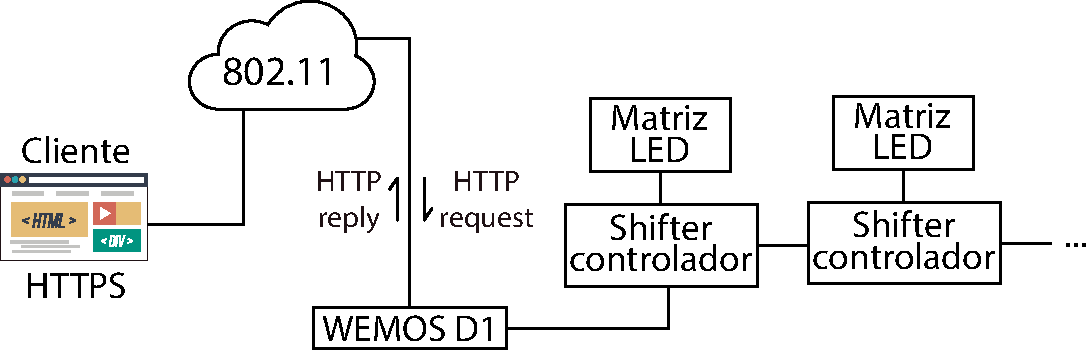
\includegraphics[width=\textwidth]{imagenes/diagrama-bloques.pdf}
            \caption{Diagrama en bloque del sistema.}
            \label{fig:diagrama-bloque}
        \end{center}
    \end{figure}


    \subsection{Comunicación entre el cliente y el Wemos D1}
    Como ya se dijo anteriormente el microcontrolador hostea una página web de manera tal que permita la comunicación entre los clientes y el Wemos D1. En la figura \ref{fig:Web-text} se observa un campo de texto para que el usuario pueda ingresar una frase, es decir caracteres alfanumericos ASCII. Cabe aclarar que las frases pueden ser elegidas como estáticas o que se desplieguen a modo de marquesina para el caso de que el mensaje supere la cantidad de módulos que se tienen. Ese campo no tiene un limite definido para la cantidad de caracteres.
    
    También, es posible especificar la velocidad en que los caracteres serán mostrados en el input inferior al de texto. Este campo esta en unidades de milisegundos y representa la velocidad que los datos de una columna de LED pasan a la siguiente columna. Si no se especifica ningún valor, los datos no se mueven.

    \begin{figure}[ht!]
    	\centering
    	\begin{center}
    		\includegraphics[width=0.9\textwidth]{imagenes/web/caracteres.png}
    		\caption{Interfaz para ingresar un texto.}
    		\label{fig:Web-text}
    	\end{center}
    \end{figure}
    
    Por otra parte, si el cliente lo desea, puede manipular los leds individualmente a través de una matriz de puntos que se encuentra en la página web. De esta forma, puede encender y apagar las luces que desee. En la figura \ref{fig:Web-matrix} se muestra la interfaz gráfica a través de la cual se implementa dicha funcionalidad. De la misma manera en que se puede controlar la velocidad de movimiento en la frase, es posible en este caso, generar un corrimiento de los estados de los LEDs.

    \begin{figure}[ht!]
    	\centering
    	\begin{center}
    		\includegraphics[width=0.8\textwidth]{imagenes/web/matriz.png}
    		\caption{Interfaz para manipular LEDs individualmente.}
    		\label{fig:Web-matrix}
    	\end{center}
    \end{figure}
    
    \vspace{5mm}
    
    Y por último, los usuarios pueden elegir diferentes secuencias animadas que se encuentran precargados en la memoria del microcontrolador; dichas animaciones se pueden observar en la figura \ref{fig:Web-predefined}.

    \begin{figure}[ht!]
    	\centering
    	\begin{center}
    		\includegraphics[width=0.8\textwidth]{imagenes/web/predef.png}
    		\caption{Interfaz para elegir imágenes precargadas en memoria.}
    		\label{fig:Web-predefined}
    	\end{center}
    \end{figure}

    La página web esta pensado para mostrarse en tanto en ordenadores de escritorio, como notebooks, tables y dispositivos móviles por lo que se desarrolló sobre un framework \emph{responsive} denominado Bootrstrap 4 Beta. En la figura \ref{fig:Web-responsive} se puede apreciar como se integra a las pantalla reducidas.

    \begin{figure}[ht!]
    	\centering
    	\begin{center}
    		\includegraphics[scale=0.7]{imagenes/web/responsive.png}
    		\caption{Interfaz para manipular LEDs en un móvil.}
    		\label{fig:Web-responsive}
    	\end{center}
    \end{figure}


    \subsection{Comunicación entre el administrador y el Wemos D1}
    El sistema provee una funcionalidad para ingresar como administrador del sitio. Esto permite realizar operaciones privilegiadas que un usuario normal no podría ejecutar. Entre ellas se destacan operaciones para eliminar la publicación actual, cambiar la intensidad de los LEDs y habilitar/deshabilitar los futuros posteos.
    
    Para acceder como administrador se debe ingresar un token de seguridad tal cual se observa en la figura \ref{fig:Web-auth}. Cabe aclarar que dicho token se corresponde con la frase ``tres tristes tigres".
    
    \begin{figure}[ht!]
    	\centering
    	\begin{center}
    		\includegraphics[width=0.7\textwidth]{imagenes/web/auth.png}
    		\caption{Interfaz para la autenticación de usuarios admin.}
    		\label{fig:Web-auth}
    	\end{center}
    \end{figure}
    
    Una vez dentro, se observa una interfaz como se muestra en la figura \ref{fig:Web-admin}. En ella se pueden observar las funcionalidades que sólo un administrador puede realizar. Las mismas se corresponden con las listadas previamente en esta sección.
    
    \begin{figure}[ht!]
    	\centering
    	\begin{center}
    		\includegraphics[width=\textwidth]{imagenes/web/admin-with-party.png}
    		\caption{Interfaz de la configuración del lado administrador.}
    		\label{fig:Web-admin}
    	\end{center}
    \end{figure}

    \subsection{Comunicación entre el Wemos D1 y el MAX7219}
    Como se detalló anteriormente, el chip shifter MAX7219 recibe una cadena de bytes de tamaño fijo vía SPI. Para ello el Wemos D1 actúa como maestro del canal e impone un clock, una señal de load y los datos que quiere transmitir (ver figura \ref{fig:Wemos-MAX}). El MAX7219 posee ocho dígitos en los cuáles almacena un byte de datos en cada uno. Para este proyecto, cada dígito representa una columna, y los datos que cada uno almacena se utilizan para representar qué filas de la columna debe encenderse. La trama del paquete se observa en la tabla \ref{table:trama-spi}.

    \begin{table}[ht]
        \centering
        \caption{Trama SPI y su significado.}
        \label{table:trama-spi}
        \begin{adjustbox}{max width=\textwidth}
        \begin{tabular}{|c|c|c|c|c|c|c|c|c|c|c|c|c|c|c|c|}
        \hline
        D15 & D14 & D13 & D12 & D11   & D10   & D9   & D8   & D7 & D6 & D5 & D4 & D3 & D2 & D1 & D0 \\ \hline
        X   & X   & X   & X   & \multicolumn{4}{c|}{ADDRESS} & \multicolumn{1}{c}{ MSB } & \multicolumn{6}{c}{ DATA } & \multicolumn{1}{c|}{ LSB } \\ \hline
        \end{tabular}
        \end{adjustbox}
    \end{table}

    En la tabla \ref{table:trama-spi} se observan los diferentes campos de interés. El primero es ADRESS que representa la columna hacia la cuál está dirigido el mensaje. El valor va desde uno hasta ocho inclusive y corresponde a las ocho columnas que tiene cada módulo. Por otra parte, DATA, representa ocho bits de información dirigida a dicha columna. Siendo D0 la fila 0 en la columna indicada por address.


    \subsection{Protocolo de comunicación SPI entre los MAX7219} \label{sec:comunicacion}
    Es importante destacar la forma en la que se comunican el microcontrolador con el primer chip shifter, y a su vez, el protocolo que utilizan para comunicarse entre los distintos MAX7219.

    La idea general consiste en indicarle a cada chip shifter los leds que debe encender y apagar en cada columna. Para ello debe enviar palabras de dos bytes de manera serial. Es decir, primero envía la información de la columna 1, después la 2, y así siguiendo hasta la 8. El protocolo utilizado es SPI y corresponde a la trama previamente detallada (ver figura \ref{table:trama-spi}).

    Para realizar este proceso, la figura \ref{fig:spi-timing-diagram} muestra un diagrama a lo largo del tiempo de la forma de enviar cada bit. En ella se puede observar que el primer paso consiste en bajar la señal de LOAD y esperar un instánte de tiempo (aproximadamente un microsegundo). Luego se debe generar una señal de CLCK de onda cuadrada y de frecuencia de 1Mhz con la mitad de ciclo de trabajo.

    El pin conectado al DATAIN del micro, se utiliza para enviar los datos, empezando por el bit más significativo primero. Los datos van a ser leídos por los MAX7219 en el flanco ascendente del CLOCK. Cuando finaliza el envio de los 16 bits, se debe subir la señal de LOAD. En ese momento, el MAX2719 almacena, en sus registros internos, el comando recibido. Todos los comandos son de dos bytes, sin embargo, se puede enviar más de esa cantidad. Esta funcionalidad se utiliza para enviar instrucciones a los demás MAX7219 que están conectados en serie. Lo que ocurre es que la información se recibe en el flanco ascendente de CLK y se envía, hacia el siguiente chip, por el pin DATAOUT en el flanco descendente. De esta forma, en una iteración se pueden configurar una columna de cada módulo de 8x8 LEDs.

    \begin{figure}[ht!]
        \centering
        \begin{center}
            \includegraphics[width=\textwidth]{imagenes/hw-conexiones/timingDiagram.pdf}
            \caption{Diagrama de tiempo de las señales del MAX7219.}
            \label{fig:spi-timing-diagram}
        \end{center}
    \end{figure}
    

    \subsection{Sucesiones de eventos}
    El sistema al iniciar, crea una red WiFi cuyo SSID corresponde a ``Remera LED'' y su password ``12345678'' (excluir las comillas). Posteriormente, monta un servidor web utilizando la dirección IP que le fue asignada, y el puerto 80. 

    Como la dirección a nivel de red podría cambiar a lo largo del tiempo, el sistema monta inmediatamente a continuación un servidor DNS que enlaza la dirección IP del servidor web con un nombre. En este caso es \enquote{\pagDNS}. Este nombre es el que deben colocar los clientes en el navegador para ingresar al sistema. El programa, tras haber iniciado el servidor DNS, se queda a la espera de las peticiones que los clientes realicen.

    El siguiente paso lo realiza el cliente. En algún momento determinado, el mismo accede a la red y coloca la contraseña. Luego abre su navegador de preferencia e ingresa al sistema escribiendo el nombre \enquote{\pagDNS}. El servidor DNS le proporciona la IP correspondiente del servicio web que hostea el microcontrolador Wemos D1.

    A partir de ese momento el usuario puede realizar alguna de las siguientes tres acciones: escribir una frase, indicar uno a uno, el estado de cada led o, incluso, elegir alguno de los sprites animados que el sistema tiene precargado en su memoria. Las figuras \ref{fig:Web-text}, \ref{fig:Web-matrix} y \ref{fig:Web-responsive} muestran, respectivamente, las páginas para realizar las acciones previamente mencionadas. Cualquiera sea la petición, el usuario puede optar por deslizar el contenido, al estilo marquesina, ingresando en el campo de texto de abajo, la velocidad por píxel que desea. El rango de valores es desde -10.000 a 10.000 milisegundos. Un valor negativo, indica que se desliza hacia la izquierda, y uno positivo hacia la derecha. Mientras que 0 indica que el mensaje no realiza desplazamiento alguno.
    
    El cliente a su vez, conociendo el token de seguridad puede acceder al sistema en modo administrador o privilegiado, tal como se muestra en la figura \ref{fig:Web-auth}. Una vez dentro, se pueden realizar cualquiera de las 4 opciones que se presentan a continuación. 
    
    En la figura \ref{fig:Web-auth} se observa una captura de pantalla de la pestaña administrador. El usuario en modo privilegiado puede eliminar la última publicación realizada presionando el botón ``clear". Adicionalmente puede cambiar la intensidad de las luces o habilitar/deshabilitar la matriz para futuras publicaciones. Cualquiera de éstas dos acciones se efectúan apretando el botón de ``Guardar". Por último, el administrador puede activar un modo fiesta haciendo click en el botón ``Party mode" que se encuentra en la esquina superior derecha de la pestaña.

    Tras haber realizado una petición, el programa, por medio del protocolo HTTP recibe los datos, los procesa y almacena los resultados en un buffer de salida. El buffer posee la información de todas las columnas a setear en la matriz. Finalmente recorre el buffer y envía serialmente cada byte por medio del protocolo SPI comenzando primero, por las columnas del último MAX7219 conectado (ver Sección \ref{sec:comunicacion}).

    La figura \ref{fig:diagrama-casos-uso} muestra un diagrama de casos de uso que representa las interacciones del cliente y de la matriz de LEDs con el sistema que corre sobre el Wemos D1, tal como se detalló previamente.

    \begin{figure}[ht!]
        \centering
        \begin{center}
            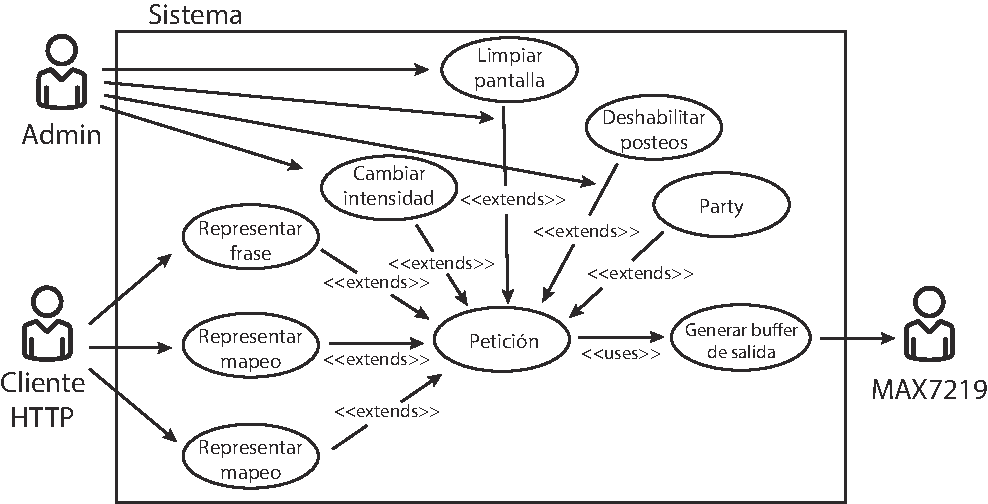
\includegraphics[width=\textwidth]{imagenes/sistema-caso-de-uso.pdf}
            \caption{Diagrama de uso de interacción ente el cliente y el driver MAX7219 con el sistema.}
            \label{fig:diagrama-casos-uso}
        \end{center}
    \end{figure}
    
    Adicionalmente en el siguiente \href{https://youtu.be/9Y2iGTpO6-U}{link} se encuentra un vídeo que muestra la secuencia completa, previamente detallada a lo largo de esta sección.



%==========================================================================================================================================================================================

\section{Descripción software}
% [Descripción de las funciones/rutinas del sistema web, asociarlas a los casos de uso o sucesiones de eventos que se describieron en la sección anterior. Agregar todo el código del sistema web como Apéndice B de este informe (usar tamaño pequeño de letra, aunque legible, y de espaciado constante o “monoespaciado” como Courier).]

% [Descripción de las funciones/rutinas del software que se ejecuta en la placa de desarrollo, asociarlas a los casos de uso o sucesiones de eventos que se describieron en la sección anterior. Agregar todo el código del software/sketch que se ejecuta en la placa de desarrollo como Apéndice C de este informe (usar tamaño pequeño de letra, aunque legible, y de espaciado constante o “monoespaciado” como Courier).]

% [Una de las mejores opciones para la descripción del software es el pseudocódigo, en el que se describen conceptualmente las operaciones del código sin llegar a copiar el código fuente propiamente dicho]

La arquitectura de software se compone de dos importantes módulos. El primero es \mbox{WebServer}, esta clase modela todas las funcionalidades relacionadas al manejo del WiFi, del servidor DNS y del servidor web. Adicionalmente se encarga de interpretar las peticiones HTTP que recibe de los clientes y enviarlas casi sin procesamiento alguno, hacia la clase Letter.

La clase Letter, corresponde al segundo módulo que compone el sistema. La misma tiene como objetivo recibir los parámetros de las peticiones y en función de los valores obtenidos, arma un buffer de salida, con la información necesaria para encender los leds correspondientes en la matriz.

En la figura \ref{fig:diagrama-bloque-sw} se observa un diagrama en bloque de los componentes de software previamente detallados, mostrando además su interacción con el exterior, es decir, con clientes y con el chip MAX7219.

\begin{figure}[ht!]
    \centering
    \begin{center}
        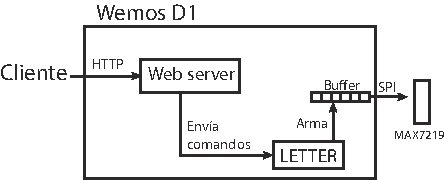
\includegraphics[width=0.8\textwidth]{imagenes/WemosD1-sistema.pdf}
        \caption{Flujo de información a través de las clases WebServer y Letter.}
        \label{fig:diagrama-bloque-sw}
    \end{center}
\end{figure}


    \subsection{Archivo principal} \label{sec:archivo-principal}
    \lstinputlisting[caption={Archivo \texttt{main.cpp}.},
                        language=C++,
                        numbers=left,
                        escapeinside={(*@}{@*)},
                        %linerange=24-57,
                        firstnumber=0]
                        {codigo/src/main.cpp}
                    
    El archivo principal o punto de entrada en este programa es el main. El trabajo que realiza es muy simple. En principio incluye las clases WebServer y Letter previamente enunciadas.

    Además tiene un método que se ejecuta una sola vez denominado setup( ) en donde inicializa los componentes de software previamente listados: WebServer y Letter. 

    A continuación un método loop( ) que se ejecuta indefinidamente. Este último permite realizar un tick a cada módulo del sistema. A lo largo de esta sección se detallan las características de cada componente mencionado. Lo importante a destacar es que la función tick( ) de cada elemento no debe ser bloqueante ni quedarse a la espera de algún evento externo que demore. Tanto el \mbox{tick( )} de WebServer como el de Letter se han implementado siguiendo esa condición.


    \subsection{Clase WebServer}
    La clase WebServer es la encargada de establecer una red WiFi, hostear un servidor DNS y uno WEB para atender las peticiones que los clientes realicen. Por otra parte, posee métodos privados para manejar cada request que se envian por medio del protocolo HTTP. 

    En primer lugar se presenta el diagrama UML de la clase WebServer. La misma se observa en la figura \ref{fig:uml-webserver} y contiene tanto los métodos públicos como privados que la clase posee.

    \begin{figure}[ht!]
        \centering
        \begin{center}
            \includegraphics[scale=1]{imagenes/WebServer.pdf}
            \caption{UML de la clase WebServer.}
            \label{fig:uml-webserver}
        \end{center}
    \end{figure}


        \subsubsection{init}
        El primer método de interés, que ya se declaró en la subsección \ref{sec:archivo-principal}, es el init( ). A continuación se presenta un pseudocódigo para comprender su funcionamiento.
    
        \lstinputlisting[caption={Pseudocódigo \texttt{WebServer.cpp}.},
                             language=C++,
                             %numbers=left,
                             escapeinside={(*@}{@*)},
                             linerange=1-9,
                             firstnumber=0]
                             {codigo/lib/WebServer/webserver.pseudo}
    
        En primer lugar se importa la librería de Arduino ``FS.h", la misma provee funcionalidades para manejar el sistema de archivos que ofrece el módulo ESP8266 dentro del Wemos D1. Este file System se denomina SPIFFS y se encuentra almacenado en una zona reservada de la flash. La cantidad de memoria depende del modelo del microcontrolador. En el caso de este proyecto es de 1MB. En el siguiente \href{https://github.com/esp8266/Arduino/blob/master/cores/esp8266/FS.h}{link} se puede acceder al código fuente de la misma.
    
        Entre las funciones que ofrece esta librería se encuentran las de leer y escribir sobre memoria no volátil. En este proyecto se utiliza para leer los archivos html almacenados en la flash a fin de msotrarlos en el navegador del cliente. Para poder utilizar estas funciones, la documentación exige que primero se ejecute la instrucción SPIFFS.begin( ).
    
        A continuación el método initWifi( ) se encarga de colocar al WemosD1 como Access Point, generar la red WiFi deseada y asignarse una dirección IP. La firma de dicha función recibe como parámetro dos punteros a char que son el nombre de la red y la contraseña.
    
        \lstinputlisting[caption={},
                         language=C++,
                         %numbers=left,
                         escapeinside={(*@}{@*)},
                         linerange=11-11,
                         firstnumber=11]
                         {codigo/lib/WebServer/webserver.pseudo}
                         
        El método initDnsServer( ) inicia un servidor DNS. Se utiliza la librería ``DNSServer.h" que corresponde al framework de Arduino. La misma provee funcionalidades para abrir un servidor DNS que corra sobre el Wemos D1, en el puerto 53. Además permite enlazar la dirección IP asignada, en el método previo, a un nombre de dominio. En nuestro caso \enquote{\pagDNS}. El código fuente de la librería puede encontrarse en el siguiente \href{https://github.com/esp8266/Arduino/blob/master/libraries/DNSServer/src/DNSServer.h}{link}.
    
        \lstinputlisting[caption={},
                         language=C++,
                         %numbers=left,
                         escapeinside={(*@}{@*)},
                         linerange=13-13,
                         firstnumber=13]
                         {codigo/lib/WebServer/webserver.pseudo}
                         
        El último método que aparece en el init( ) de la clase WebServer, es initWebServer( ). Éste es el que se encarga propiamente de iniciar un servidor web, en el puerto 80.
        
        \lstinputlisting[caption={},
                         language=C++,
                         %numbers=left,
                         label = frag:initWebServer,
                         escapeinside={(*@}{@*)},
                         linerange=16-34,
                         firstnumber=16]
                         {codigo/lib/WebServer/webserver.pseudo}
    
        Inicialmente se incluye la librería ``ESP8266WebServer.h" la misma provee funcionalidades para iniciar y manejar un servidor web. Los métodos utilizados en el proyecto se explican a lo largo de esta sección.
        
        En primer lugar se instancia un objeto del tipo ESP8266WebServer, esta clase es la que tiene las funciones que proporciona la librería previamente mencionada. El constructor toma un parámetro que es el puerto donde se van a escuchar las conexiones. En nuestro caso el 80.
        
        El siguiente método es on( ). Éste permite enlazar una petición a un callback, es decir que cuando el cliente realice una acción, por ejemplo un GET REQUEST, se ejecuta la función especificada en el método on( ). En el fragmento \ref{frag:initWebServer} se puede observar que los callbacks que se pasan como parámetros corresponden a los métodos privados de la clase WebServer (ver figura \ref{fig:uml-webserver}). Su funcionamiento se detalla en la sección que se encuentra a continuación.
    
        Posterior a la etapa de configuración, la librería ``ESP8266WebServer.h" posee un método para iniciar efectivamente el server y permitir que los clientes accedan a él. Eso se realiza ejecuntando la función begin( ).
                         
    
        \subsubsection{httpHandlers}
        En la sección anterior se mencionó que la clase WebServer posee diferentes métodos privados denominados callbacks. Éstos se ejecutan ante las diferentes peticiones HTTP que el cliente realiza a través del servidor web hosteado por el Wemos D1 (ver figura \ref{fig:uml-webserver}).
    
        Estos callbacks se clasifican en dos: los que antienden peticiones del tipo GET y los que son del tipo POST. La declaración de sus encabezados permite identificar al grupo al que pertenece cada uno. Por ejemplo handleGetIndex( ) y handlePostMatrix( ). El primero se ejecuta cuando se accede a la dirección ``/index'' a través de un HTTP GET REQUEST mientras que el segundo cuando se accede a ``/matrix" por POST. El comportamiento es muy similar de acuerdo a la categoría donde pertenecen. En este apartado se explica en pseudocódigo las dos categorías previamente enunciadas para estos callbacks.
    
        En primer lugar se explica el comportamiento de los callbacks privados de la clase WebServer que son del tipo GET. Se puede observar que la implementación es muy simple. Cuando se pida ``/index" por GET, se va a usar la librería FS.h previamente descripta para cargar en RAM el archivo index.html alojado en la memoria no volátil del microcontrolador.
    
        Luego se envía el HTML como respuesta, hacia el cliente con la respuesta 200 que significa OK. El fragmento \ref{fig:cbGet} muestra el pseudocódigo del comportamiento del callback del tipo GET.
    
        \lstinputlisting[caption={Pseudocódigo de un callback del tipo GET},
                         language=C++,
                         %numbers=left,
                         escapeinside={(*@}{@*)},
                         label = fig:cbGet,
                         linerange=36-40,
                         firstnumber=36]
                         {codigo/lib/WebServer/webserver.pseudo}
    
        Para el caso de un callback de la categoría POST (ver pseudocódigo del fragmento \ref{fig:cbPost}), en primer lugar se realiza la obtención de los argumentos enviados por parte del cliente. Se realiza el procesamiento de esos argumentos, luego se obtiene el archivo HTML que corresponde y se envia por el socket establecido con el usuario cuya respuesta posee el valor 200.
        % El fragmento \ref{fig:cbPost} se puede observar un pseudocódigo de lo detallado en este párrafo.
    
        La acción de procesar los argumentos, consiste en determinar qué tipo de pedido está realizando el cliente. Recordar las tres categorías de los mismos: publicar una frase, representar un sprite animado o determinar led a led el estado de cada uno. 
        
        Adicionalmente el administrador puede realizar cualquiera de las siguiente 4 opciones: eliminar la última publicación, habilitar/deshabilitar posteos, cambiar la intensidad de los LEDs y activar el modo fiesta.
        
        Una vez que se conoce cuál es el pedido, se ejecuta el método de la clase Letter correspondiente para que envíe la información vía SPI a los MAX7219.
                         
        \lstinputlisting[caption={Pseudocódigo de un callback del tipo POST},
                         language=C++,
                         %numbers=left,
                         escapeinside={(*@}{@*)},
                         label = fig:cbPost,
                         linerange=42-49,
                         firstnumber=42]
                         {codigo/lib/WebServer/webserver.pseudo}
                         
                         
        \subsubsection{tick}
        Se debe recordar que en la sección \ref{sec:archivo-principal}, en el archivo principal, se describe un método denominado loop( ). En cada llamdo, se realiza un tick a cada componente de software que integran el sistema por lo tanto resulta fundamental que dicha función sea no-bloqueante.
    
        La clase WebServer implementa el método tick( ) (ver UML de la figura \ref{fig:uml-webserver}) y en su cuerpo simplemente se encarga de ejecutar la función handleClient de la librería ``ESP8266WebServer.h'' previamente mencionada. En el siguiente \href{https://github.com/esp8266/Arduino/blob/master/libraries/ESP8266WebServer/src/ESP8266WebServer.h}{link} se puede observar la documentación completa. Sin embargo alcanza con saber que su principal tarea es comprobar si algún cliente ha realizado alguna petición HTTP. En caso de que la respuesta sea afirmativa, ejecuta el callback correspondiente, si no, retorna inmediatamente sin realizar acción alguna.
    
        \lstinputlisting[caption={},
                         language=C++,
                         %numbers=left,
                         escapeinside={(*@}{@*)},
                         linerange=51-51,
                         firstnumber=51]
                         {codigo/lib/WebServer/webserver.pseudo}
                         
                         
    \subsection{Clase Letter}
    La clase Letter es el segundo módulo de software más importante en la solución de este problema. Su principal función consiste en recibir los datos que le pasa por parámetro la clase WebServer, procesarlos y armar un buffer de salida con la información necesaria para encender las luces de la matriz. Para la comunicación con los MAX7219 se utiliza el protocolo de transmisión SPI como se observa en la figura \ref{fig:diagrama-bloque-sw}.

    Los métodos que componen la clase se describen en el diagrama UML de la figura \ref{fig:uml-letter}. Se puede observar que las funciones públicas son init( ) y tick( ) al igual que en WebServer. Cabe recordar, que este último método no debe ser bloqueante ni quedarse a la espera de un evento asíncrónico externo. En cualquier caso, si no cuenta con la información necesaria para ejecutar ciertas acciones, debe retornar inmediatamente.

    \begin{figure}[ht!]
        \centering
        \begin{center}
            \includegraphics[scale=1]{imagenes/Letter.pdf}
            \caption{UML de la clase Letter.}
            \label{fig:uml-letter}
        \end{center}
    \end{figure}


        \subsubsection{init}
        El método init( ) se encarga de configurar todos los registros necesarios del MAX7219 para iniciar su funcionamiento. Entre las acciones que realiza, el programa se encarga de sacarlo del modo test, setearle la intensidad de los leds, indicarle que se van a usar las ocho columnas que posee el chip, limpiarle la pantalla apagando todos los leds y encenderlo. En el fragmento \ref{fig:letter-init} se observa un pseudocódigo de la etapa de inicialización de los registros del MAX7219 para configurarlo de la manera detallada anteriormente.

        \lstinputlisting[caption={Pseudocódigo del método init de la clase Letter.cpp},
                     language=C++,
                     %numbers=left,
                     escapeinside={(*@}{@*)},
                     label = fig:letter-init,
                     linerange=1-13,
                     firstnumber=1]
                     {codigo/lib/Letter/letter.pseudo}

        En primer lugar se incluye la librería ``SPI.h". La misma corresponde al framework de Arduino y se puede consultar su documentación completa en el siguiente \href{https://github.com/arduino/Arduino/blob/master/hardware/arduino/avr/libraries/SPI/src/SPI.h}{link}. Su función principal es abstraer el manejo del protocolo de transmisión serial, a partir de determinadas funciones que la librería provee. Para comenzar a utilizarla se debe ejecutar el método SPI.begin( ).
    
        Las siguientes instrucciones consisten en configurar todos los MAX7219 a través del método sendCommand( ). La función toma dos parámetros, en el primero se especifica el registro a configurar y en el segundo el valor que se desea establecer. Para más información respecto de la configuración de los registros consultar el datasheet del MAX7219 haciendo click en el siguiente \href{https://datasheets.maximintegrated.com/en/ds/MAX7219-MAX7221.pdf}{link}.

        \subsubsection{Método setMessage}
        El siguiente método público que aparece en el diagrama UML de la figura \ref{fig:uml-letter} es \mbox{setMessage( )}. Esta función es la encargada de procesar las peticiones relacionadas a las frases que el usuario publica en la matriz (ver el diagrama de casos de uso de la figura \ref{fig:diagrama-casos-uso}). El método recibe tres parámetros. En primer lugar el mensaje a setear en la matriz de LEDs. La longitud máxima del mensaje a representar está definido por la variable global MESSAGE SIZE.

        El siguiente parámetro es strLen, este valor indica la cantidad de caracteres que posee el string message. No debe incluirse el caracter nulo ni tampoco superar el valor de la variable \mbox{MESSAGE SIZE}.

        El último parámetro de interés es srate. Su valor indica la velocidad por píxel al que se debe mover el mensaje. Acepta valores negativos y en ese caso el contenido se desliza hacia la izquierda. Caso contrario hacia la derecha.

        El comportamiento de este método es muy simple. Toma el mensaje que se recibe, y busca la representación de cada carácter en un arreglo que el microcontrolador posee. Ese arreglo le indica los valores que tiene que enviar a las diferentes columnas de la matriz para representar cada letra. Cada valor es cargado en orden en el búffer de salida.

        \lstinputlisting[caption={},
                     language=C++,
                     %numbers=left,
                     escapeinside={(*@}{@*)},
                     %label = fig:letter-init,
                     linerange=16-18,
                     firstnumber=16]
                     {codigo/lib/Letter/letter.pseudo}

        \subsubsection{setMap}
        Este método es el encargado de procesar las peticiones cuando el usuario quiere encender y apagar determinados LEDs de manera individual (ver el diagrama de casos de uso de la figura \ref{fig:diagrama-casos-uso}). El método recibe tres parámetros. 
        En primer lugar un arreglo de bytes donde cada posición representa una columna de la matriz de LEDs y el valor (el byte en esa posición del vector) indica qué leds deben encenderse y cuáles no. Siendo el bit menos significativo la fila cero de la columna en cuestión.
        El segundo parámetro es la cantidad de columnas a setear. La misma no puede exceder \mbox{\texttt{MAX LETTERS * 8}}. Si no el comportamiento se torna indefinido. En caso de que el tamaño fuese menor que la cantidad de matrices que hay, se rellena con columnas en 0. Es decir, apagadas.
        El último valor es srate. Su valor indica la velocidad por píxel al que se debe mover el contenido.
        El comportamiento de este método consiste en tomar el arreglo de columnas que se recibe por parámetro y copiar dichos valores en el buffer de salida. De esta forma la información queda lista para ser enviada bajo el protocolo de SPI.
        
        \lstinputlisting[caption={},
                         language=C++,
                         %numbers=left,
                         escapeinside={(*@}{@*)},
                         %label = fig:letter-init,
                         linerange=20-22,
                         firstnumber=20]
                         {codigo/lib/Letter/letter.pseudo}
                   
                             
        \subsubsection{setPredefined}
        Este método se asocia con el caso de uso relacionado a que el usuario puede elegir representar en la matriz de LEDs una serie de sprites animados previamente cargados en la flash del microcontrolador Wemos D1 (ver el diagrama de casos de uso de la figura \ref{fig:diagrama-casos-uso}). El método recibe dos parámetros. El primero corresponde con un enumerativo que determina cuál de todos los sprites precargados se quiere representar. En caso de que se enviara información que no corresponda con ningún sprite, la función retorna inmediatamente. Actualmente los sprites precargados son una sonrisa, un pacman y un corazón animado.
        
        El segundo parámetro es srate. Su valor indica la velocidad por píxel al que se debe mover el sprite. Acepta valores negativos y en ese caso el contenido se desliza hacia la izquierda. Caso contrario hacia la derecha.
        
        El comportamiento de este método consiste en analizar qué sprite se quiere representar, almacenar dicha información en una variable interna y luego llenar el buffer de salida con la información precargada que se tiene de ese sprite. Dichos datos corresponden a los leds que se deben encender en cada columna de la matriz a fin de representar el sprite determinado por el usuario.

        \lstinputlisting[caption={},
                     language=C++,
                     %numbers=left,
                     escapeinside={(*@}{@*)},
                     %label = fig:letter-init,
                     linerange=24-26,
                     firstnumber=24]
                     {codigo/lib/Letter/letter.pseudo}
                     
                     
        \subsubsection{setPartyOn}
        Este método provee funcionalidad para encender aleatoriamente las luces de la matriz de un modo divertido. Se diseñó especialmente para la demostración del proyecto y tampoco recibe ningún paramétro extra.
        El comportamiento consiste en llenar el buffer de salida con números generados aleatoriamente con la función de Arduino random( ). Los números van desde 0 a 255 inclusive y representa todas las combinaciones de estados que pueden tomar los LEDs. Siendo 0 todos apagados y 255 todos encendidos. Cada cierto intervalo de tiempo, se renueva los valores del buffer de salida enviando los nuevos estados de los LEDs.
        
        \lstinputlisting[caption={},
                     language=C++,
                     %numbers=left,
                     escapeinside={(*@}{@*)},
                     %label = fig:letter-init,
                     linerange=30-30,
                     firstnumber=30]
                     {codigo/lib/Letter/letter.pseudo}
                     
        
        \subsubsection{setEnabled}
        El funcionamiento de este método consiste en habilitar o deshabilitar las publicaciones que se realicen a la matriz. Recibe un solo parámetro booleano que determina si el sistema acepta nuevas publicaciones. Un valor falso indica que no se pueden enviar nuevos posteos hasta que el flag de enabled vuelva a ser verdadero.
        
        \lstinputlisting[caption={},
                     language=C++,
                     %numbers=left,
                     escapeinside={(*@}{@*)},
                     %label = fig:letter-init,
                     linerange=32-32,
                     firstnumber=32]
                     {codigo/lib/Letter/letter.pseudo}
        
        
        \subsubsection{setIntensity}
        Este método provee funcionalidad para cambiar, en tiempo real, la intensidad con la que se encienden los LEDs de la matriz. 
        
        Recibe un parámetro de configuración que es un número representado en 8 bits sin signo. El mismo especifica el brillo de las luces y va desde 0 hasta 15 inclusive. En caso de que se introduzca un número superior, se tomarán los 4 bits menos significativos del parámetro.
        
        \lstinputlisting[caption={},
                     language=C++,
                     %numbers=left,
                     escapeinside={(*@}{@*)},
                     %label = fig:letter-init,
                     linerange=34-34,
                     firstnumber=34]
                     {codigo/lib/Letter/letter.pseudo}
                     
        
        \subsubsection{clearScreen}
        Esta funcionalidad de la clase Letter se utiliza para limpiar el último posteo que realizó el cliente, limpiando el buffer de salida. A fin de eliminar la publicación actual, se coloca cero en cada índice del arreglo del buffer. Luego se envía esa información a cada columna de la matriz.
        
        El método no posee argumentos.
        
        \lstinputlisting[caption={},
                     language=C++,
                     %numbers=left,
                     escapeinside={(*@}{@*)},
                     %label = fig:letter-init,
                     linerange=36-36,
                     firstnumber=36]
                     {codigo/lib/Letter/letter.pseudo}
                     
                     
        \subsubsection{tick}
        Se debe recordar que el método tick( ) de la clase Letter es llamado sólo en el archivo principal main.cpp en su función loop( ). El funcionamiento es muy simple, y solo tiene sentido cuando se elige una velocidad de desplazamiento del contenido distinta a cero. La clase Letter posee determinadas variables internas que le permiten saber cuál es el primer índice del buffer de salida que se debe enviar por serial hacia los MAX7219.

        El método, entonces, determina si la velocidad por píxel es positiva o negativa y en función del resultado mueve el índice hacia la izquierda o derecha respectivamente. Luego actualiza la información de los shifters para que representen la nueva imagen desplazada.

        \lstinputlisting[caption={},
                     language=C++,
                     %numbers=left,
                     escapeinside={(*@}{@*)},
                     %label = fig:letter-init,
                     linerange=28-28,
                     firstnumber=28]
                     {codigo/lib/Letter/letter.pseudo}


\clearpage

%==========================================================================================================================================================================================

\section{Guías}
    % [Siguiendo esta guía paso a paso debería ser posible reconstruir el proyecto completo casi sin conocimientos previos de los detalles involucrados. Esta guía es esencial no solamente para reconstruir el proyecto sino para su continuación/evolución]
    
    
    \subsection{Ambiente de desarrollo e instalación}
    % [Debería documentarse desde la instalación de drivers necesarios hasta el software de desarrollo (IDE y/o lenguajes necesarios) y lo desarrollado (programas fuente), para que el proyecto se pueda reproducir, mantener, modificar, mejorar y/o agregar funcionalidad, etc. A partir de lo documentado en esta sección debería ser posible que otro grupo de trabajo retome el proyecto a partir de lo entregado. En el caso de los programas fuente, no incluir el listado, solamente la enumeración de lo desarrollado y en qué ambiente debería ser utilizado. En el caso de software que no sea de proveedores conocidos o que tengan alguna posibilidad de no mantenerse en los sitios web, descargarlos y adjuntarlos al presente informe. Arduino es un ejemplo de sitio que ha perdurado en el tiempo, con lo cual no sería necesario]
    
    Para los requisitos que se listan a continuación se recomienda utilizar el sistema operativo GNU/Linux. Cabe destacar que el presente proyecto se realizó sobre máquinas con la distribución Ubuntu 16.04.
    
    
        \subsubsection{Git}
        En primer lugar se necesita la herramienta de software denominada git. La misma está disponible tanto para Linux, como para Windows y macOS. La instalación se puede realizar a través de un instalador binario, en general se utiliza la herramienta básica de administración de paquetes que trae la distribución. En el caso de distribución basada en Debian como Ubuntu, se puede utilizar \texttt{apt-get}.
        
        \lstinputlisting[caption={},
                     language=bash,
                     %numbers=left,
                     escapeinside={(*@}{@*)},
                     %label = fig:letter-init,
                     linerange=1-1,
                     firstnumber=1]
                     {codigo/instalacion/instalacion.pseudo}
        
        En caso de un ambiente Windows, se recomienda utilizar \href{https://git-for-windows.github.io}{git bash}. Mientras que para computadoras con sistema operativo macOS se recomienda descargar la imagen en el siguiente \href{https://git-scm.com/download/mac}{link}.
        
        
        \subsubsection{Visual Studio Code}
        A continuación se requiere el editor Visual Studio Code. El mismo se puede descargar de su página principal, haciendo click \href{https://code.visualstudio.com/Download}{aquí}. Luego se debe elegir la extensión de acuerdo al sistema operativo que se desee. Una vez descargado el archivo, se debe descomprimir su contenido y almacenarlo en alguna carpeta determinada. En el caso de linux, ejecutar el siguiente comando.

        \lstinputlisting[caption={},
                     language=bash,
                     %numbers=left,
                     escapeinside={(*@}{@*)},
                     %label = fig:letter-init,
                     linerange=2-2,
                     firstnumber=2]
                     {codigo/instalacion/instalacion.pseudo}
        
        Lo que hace este comando es descomprimir el contenido del archivo VSCode-linux-x64.zip en la carpeta /opt/vscode. Con el parámetro -d se indica que cree la carpeta en caso de que no exista. 
        
        Para ejecutar el programa, se necesita acceder a la carpeta donde se descargó el contenido y luego escribir ./Code.
        
        \lstinputlisting[caption={},
                     language=bash,
                     %numbers=left,
                     escapeinside={(*@}{@*)},
                     %label = fig:letter-init,
                     linerange=3-4,
                     firstnumber=3]
                     {codigo/instalacion/instalacion.pseudo}
        
        Adicionalmente si se quiere tener un acceso directo al escritorio, se debe dirigir a la carpeta donde se descargó el programa, en este caso /opt/vscode y abrir con algún editor de texto con la extensión .desktop. Allí dentro añadimos el siguiente contenido.
        
        \lstinputlisting[caption={},
                     language=bash,
                     %numbers=left,
                     escapeinside={(*@}{@*)},
                     %label = fig:letter-init,
                     linerange=5-11,
                     firstnumber=5]
                     {codigo/instalacion/instalacion.pseudo}
        
        
        \subsubsection{Plugins necesarios para Visual Studio Code}
        Para el desarrollo de este proyecto se requirió la instalación de los plugins que se listan a continuación en el orden en que son mencionados.
        
        \begin{itemize}
            \item \href{https://marketplace.visualstudio.com/items?itemName=ms-vscode.cpptools}{C++}.
            \item \href{https://marketplace.visualstudio.com/items?itemName=webfreak.debug}{Native Debug}.
            \item \href{https://marketplace.visualstudio.com/items?itemName=platformio.platformio-ide}{PlatformIO IDE}.
        \end{itemize}
        
        Para la instalación se puede ingresar en los diferentes links listados, los cuales abrirán una página web y presionando en el botón instalar, automáticamente se añadirá la extensión a Visual Studio Code.
        
        Otra forma de agregar los plugins es abriendo el programa y seleccionado, en la barra de tareas, la pestaña ver-> extensiones. Esto desplegará un campo de texto donde se debe escribir el nombre de la extensión a instalar. En nuestro caso se deben ingresar, en mismo orden, los nombres de los plugins listados al inicio de esta sección y apretar en el botón instalar.
    
        
    \subsection{Instalación}
    % % [Identificar qué archivos corresponden a qué hardware o subsistema (ej: web en la PC y sketch en Arduino). Cada una de estos archivos deben ser adjuntados al presente informe. Notar que el mismo software se ha incorporado en/como Apéndices, pero en este caso debe ser adjuntado (como directorio/s y/o archivo/s en .zip o .tar.gz) con el objetivo de ser reconstruido el sistema de desarrollo]
    Todos los archivos fuente que se encuentran en los apéndices B y C, corresponden al programa que se ejecuta dentro del Wemos D1. En este proyecto no se utiliza la PC como parte del sistema.
    
    A fin de brindar más claridad a esta sección se listan todos los nombres de los archivos que se agregan en el microcontrolador. En sus respectivas carpetas (ver listado de la figura \ref{fig:tree-code}).
    
    \begin{figure}[ht!]
        \begin{center}
        \begin{forest}
          for tree={folder, grow'=0, fit=band,}
            [/
                [main.cpp]
                [lib/
                    [WebServer/
                        [WebServer.h]
                        [WebServer.cpp]
                    ]
                    [Letter/
                        [Letter.h]
                        [Letter.cpp]
                    ]
                ]
                [data/
                    [static/
                        [favicon.png.gz]
                    ]
                    [admin.html.gz]
                    [authentication.html.gz]
                    [config.html.gz]
                ]
            ]
        \end{forest}
        \end{center}
        \caption{Árbol de archivos del proyecto.}
        \label{fig:tree-code}
    \end{figure}
        

    \subsection{Compilación}
    % [Indicar configuraciones y ubicaciones de los ejecutables y código del sistema en el caso del subsistema web y si hay alguna consideración o configuración especial para el código que se ejecute en la placa de desarrollo]
    Se decidió confeccionar un video ilustrativo que muestre los pasos ordenados que se deben realizar a fin de poder reproducir el proyecto. El enlace se encuentra en el haciendo click en el siguiente \href{https://www.youtube.com/watch?v=lrKF8X2M1RY&feature=youtu.be}{link}. Adicionalmente, se listan los pasos a continuación de forma que se complementen con el video.
    
    En primer lugar se debe clonar el repositorio: \url{https://github.com/trorik23/tpii.git} ejecutando el siguiente comando
    
    \lstinputlisting[caption={},
                     language=C++,
                     %numbers=left,
                     escapeinside={(*@}{@*)},
                     %label = fig:letter-init,
                     linerange=12-12,
                     firstnumber=12]
                     {codigo/instalacion/instalacion.pseudo}
    
    Posteriormente se debe acceder a la carpeta \emph{web} dentro del repositorio, en él se encontrara un srcipt llamado \emph{scrip.sh}. Una vez localizado, se debe ejecutar el script: \texttt{./script.sh}, esto hará que se carguen los archivos html (comprimidos con gzip) dentro de la carpeta \emph{wemos/data} listo para ser flasheado al Wemos D1.
    
    \lstinputlisting[caption={},
                     language=C++,
                     %numbers=left,
                     escapeinside={(*@}{@*)},
                     %label = fig:letter-init,
                     linerange=13-14,
                     firstnumber=13]
                     {codigo/instalacion/instalacion.pseudo}
    
    Para realizar pasos listados a continuación, se debe conectar el Wemos D1 a la PC de desarrollo y abrir Visual Studio Code.
    \begin{itemize}
        \item En home de PlatformIO seleccionar \enquote{Open Project} y buscar la carpeta \enquote{wemos} (donde se encuentra el archivo \texttt{platformio.ini}).
        \item Dentro de Visual Studio Code, con el proyecto ya importado, seleccionar abajo a la izquierda, el ícono \enquote{PlatformIO: Run a Task}.\\
        Eso desplegará una serie de funcionalidades que se pueden realizar con el Wemos D1. Ahí se debe elegir \enquote{PlatformIO: Upload SPIFFS Image}. Eso cargará en la memoria del micro los archivos HTML que utilizará el servidor web.\\
        Este paso solo debe repetirse cada vez que se modifique los archivos HTML.\\
        ACLARACIÓN: El proceso de cargar en la SPIFFS del Wemos D1 se realiza mediante serial por lo que no se puede estar ejecutando ninguna otra tarea que involucre serial tales como \enquote{SerialMonitor} o \enquote{Upload}.
        \item Una vez cargada los archivos HTML, ingresar en la opción \enquote{Build}.
        \item Si la compilación del paso anterior fue exitosa, realizar la tarea de \enquote{Upload} que se encuentra en las opciones anteriormente mencionadas o en la barra inferior izquierda haciendo click sobre el icono de la flecha.\\
        ACLARACIÓN: Cada vez que se modifique el programa se debe rehacer los últimos dos paso.
    \end{itemize}